%%%%%%%%%%%%%%%%%%%%%%%%%%%%%%%%%%%%
% Slide options
%%%%%%%%%%%%%%%%%%%%%%%%%%%%%%%%%%%%

% Option 1: Slides with solutions

\documentclass[t,compress,mathserif]{beamer}
\newcommand{\soln}[1]{\textit{#1}}
\newcommand{\solnGr}[1]{#1}

% Option 2: Handouts without solutions

%\documentclass[11pt,containsverbatim,handout]{beamer}
%\usepackage{pgfpages}
%\pgfpagesuselayout{4 on 1}[letterpaper,landscape,border shrink=5mm]
%\newcommand{\soln}[1]{ }
%\newcommand{\solnGr}{ }


%%%%%%%%%%%%%%%%%%%%%%%%%%%%%%%%%%%%
% Style
%%%%%%%%%%%%%%%%%%%%%%%%%%%%%%%%%%%%

\def\chpiv@path{../../Chp 4}
\def\chpv@path{../../Chp 5}
\input{../../lec_style.tex}

%%%%%%%%%%%%%%%%%%%%%%%%%%%%%%%%%%%%
% Preamble
%%%%%%%%%%%%%%%%%%%%%%%%%%%%%%%%%%%%

\title[Lecture 17]{MA213: Lecture 17}
\subtitle{Module 3: Foundations for inference}
\author{OpenIntro Statistics, 4th Edition}
\institute{$\:$ \\ {\footnotesize Based on slides developed by Mine \c{C}etinkaya-Rundel of OpenIntro. \\
The slides may be copied, edited, and/or shared via the \webLink{http://creativecommons.org/licenses/by-sa/3.0/us/}{CC BY-SA license.} \\
Some images may be included under fair use guidelines (educational purposes).}}
\date{}


%%%%%%%%%%%%%%%%%%%%%%%%%%%%%%%%%%%%
% Begin document
%%%%%%%%%%%%%%%%%%%%%%%%%%%%%%%%%%%%

\begin{document}

%%%%%%%%%%%%%%%%%%%%%%%%%%%%%%%%%%%%
% Title page
%%%%%%%%%%%%%%%%%%%%%%%%%%%%%%%%%%%%

{
\addtocounter{framenumber}{-1} 
{\removepagenumbers 
\usebackgroundtemplate{\includegraphics[width=\paperwidth]{../../OpenIntro_Grid_4_3-01.jpg}}
\begin{frame}

    \hfill \includegraphics[width=20mm]{../../oiLogo_highres}
    \titlepage

\end{frame}
}
}

\begin{frame}
    \frametitle{Module 3: Foundations for inference}
    \begin{itemize}
        \item \hl{Previously: }Point estimates and sampling variability (Chapter 5.1)
        \item \hl{This time: }Confidence intervals (Chapter 5.2)
        \item \hl{Reading: }Chapter 5.3 for next time
        \item \hl{Deadlines/Announcements: }
        \begin{itemize}
            \item HW 6 due on Tuesday
            \item Reminder: Monday is a Holiday, Tuesday is Monday schedule
            \item Quiz 2 \hl{in class on Wednesday}, \textbf{Not in discussion sections}
            \item No discussion sections next week
        \end{itemize}
    \end{itemize}
    
\end{frame}
    
%%%%%%%%%%%%%%%%%%%%%%%%%%%%%%%%%%%%
% Learning objectives:
%%%%%%%%%%%%%%%%%%%%%%%%%%%%%%%%%%%%
\begin{frame}
\frametitle{Learning Objectives}
\begin{itemize}
    \item \textbf{M3 LO3: Calculate and Interpret Standard Error:} Calculate the standard error for proportions and interpret it as a measure of sampling variability. 
    \item \textbf{M3 LO4: Explain Hypothesis Testing and Its Limitations:} Discuss the use cases and potential issues with hypothesis testing, including the interpretation of results. 
    \item \textbf{M4 LO1: Design and Interpret Confidence Intervals:} Design, execute, and interpret confidence intervals for the population proportion. 
\end{itemize}
\end{frame}


%%%%%%%%%%%%%%%%%%%%%%%%%%%%%%%%%%%%
% Sections
%%%%%%%%%%%%%%%%%%%%%%%%%%%%%%%%%%%%

\begin{frame}
\frametitle{Sampling distribution of the sample proportion}
    \begin{itemize}
        \item For a sample of size $n$ and population proportion $p$, the number of successes $X \sim \text{Binomial}(n, p)$
        \item The sample proportion is a rescaled version of $X$: $\hat{p} = \frac{X}{n}$
        \item So the sampling distribution of $\hat{p}$ is just like the binomial distribution, but for values from $0$ to $1$ instead of $0$ to $n$
    \end{itemize}
    \vspace{2em}
    \begin{columns}[T] 
        \begin{column}{0.4\textwidth}
            \vspace{2em} 
            \footnotesize{\textcolor{red}{Note:} Assumes that the population is much larger than the sample, so that sampling with replacement is a good approximation to sampling without replacement.}
        \end{column}
        \begin{column}{0.6\textwidth}
            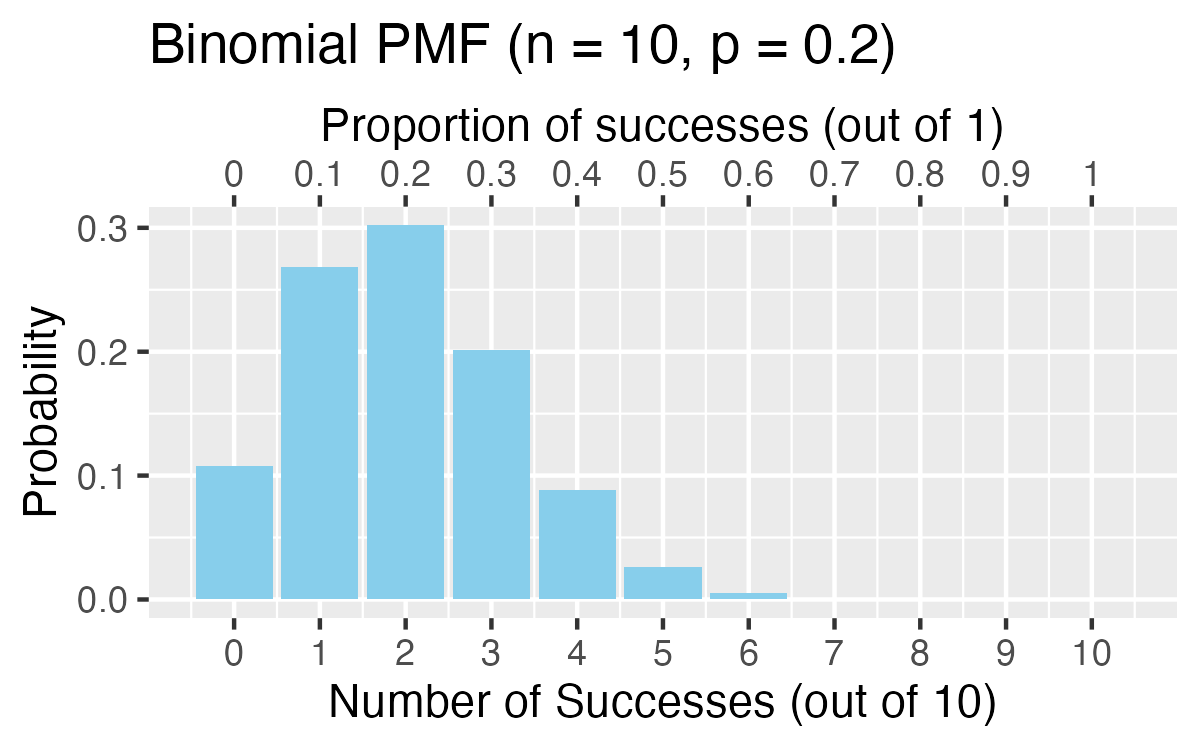
\includegraphics[width=\textwidth]{../Lecture16/sampling_dist_of_phat.png}
        \end{column}
    \end{columns}
\end{frame}

%%%%%%%%%%%%%%%%%%%%%%%%%%%%%%%%%%%

\begin{frame}
\frametitle{Sampling distribution of the sample proportion}

$X \sim \text{Binomial}(n, p)$ \\
$\hat{p}  = \frac{X}{n}$ \\

\vspace{1em}
\textcolor{orange}{$Pr(\hat{p}  = \frac{k}{n}) = Pr(X = k) = \dbinom{n}{k} p^k (1-p)^{n-k}$} \\
for $\frac{k}{n} \in \left\{0, \frac{1}{n}, \frac{2}{n}, \ldots, \frac{n-1}{n}, 1\right\}$


This is the theoretical \hl{sampling distribution} of $\hat{p}$!
\end{frame}
%%%%%%%%%%%%%%%%%%%%%%%%%%%%%%%%%%%%

\begin{frame}
\frametitle{Normal approximation to the Binomial}

When the sample size is large enough ($np \ge 10$  and  $n(1-p) \ge 10$), the binomial distribution with parameters $n$ and $p$ can be approximated by the normal model with parameters $\mu = np$ and $\sigma = \sqrt{np(1-p)}$.

\[Binomial(n,p) \approx Normal(\mu = np, \sigma = \sqrt{np(1-p)})\]

\begin{center}
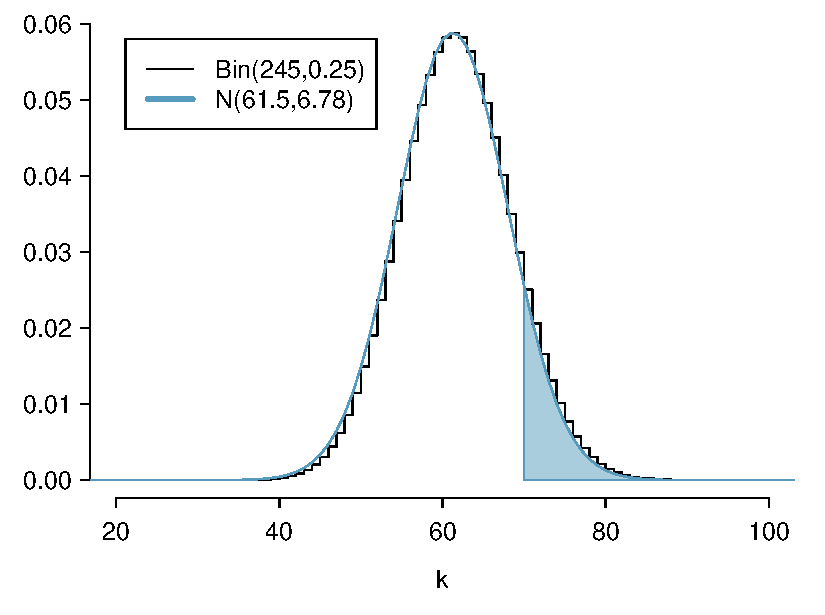
\includegraphics[width=0.5\textwidth]{\chpiv@path/4-3_binomial_distribution/figures/fb_power_user/fb_power_user}
\end{center}

\end{frame}

%%%%%%%%%%%%%%%%%%%%%%%%%%%%%%%%%%%%%

\section{Central Limit Theorem (Ch. 5.1-5.2)}

%%%%%%%%%%%%%%%%%%%%%%%%%%%%%%%%%%%%

\section{R Demo: For large samples, does the sample proportion also have a Normal sampling distribution? }

%%%%%%%%%%%%%%%%%%%%%%%%%%%%%%%%%

\begin{frame}
\frametitle{Central Limit Theorem}

\formula{Central limit theorem (sample proportion)}
{Sample proportions will be nearly normally distributed with mean equal to the population proportion, $p$, and standard error equal to $\sqrt{\frac{p~(1-p)}{n}}$.
\[ \hat{p} \sim N \pr{ mean = p, SE = \sqrt{\frac{p~(1-p)}{n}} } \]
}

\begin{itemize}

\item This comes from the fact that the Binomial distribution converges to the Normal distribution as $n$ increases.
\item The standard error $SE =  \sqrt{\frac{p~(1-p)}{n}}$ is what we derived on the board for $\hat{p}$. Note that as $n$ increases $SE$ decreases.
\begin{itemize}
\item As $n$ increases samples will yield more consistent $\hat{p}$s, i.e. variability among $\hat{p}$s will be lower.
\end{itemize}

\end{itemize}

\end{frame}

%%%%%%%%%%%%%%%%%%%%%%%%%%%%%%%%%%%%

\begin{frame}
\frametitle{CLT - conditions}

Certain conditions must be met for the CLT to apply:

\begin{enumerate}

\item \hlGr{Independence:} Sampled observations must be independent. \\

This is difficult to verify, but is more likely if
\begin{itemize}
\item random sampling/assignment is used, and
\item if sampling without replacement, $n$ $<$ 10\% of the population.
\end{itemize}

\pause

\item \hlGr{Sample size:} There should be at least 10 expected successes and 10 expected failures in the observed sample.

This is difficult to verify if you don't know the population proportion (or can't assume a value for it). In those cases we look for the number of observed successes and failures to be at least 10.

\end{enumerate}

\end{frame}

%%%%%%%%%%%%%%%%%%%%%%%%%%%%%%%%%%

\begin{frame}
\frametitle{When $p$ is unknown}

\begin{itemize}

\item The CLT states $SE = \sqrt{\frac{p~(1-p)}{n}}$, with the condition that $np$ and $n(1-p)$ are at least 10, however we often don't know the value of $p$, the population proportion

\item In these cases we substitute $\hat{p}$ for $p$

\end{itemize}

\end{frame}

%%%%%%%%%%%%%%%%%%%%%%%%%%%%%

\section{Edfinity quiz}

%%%%%%%%%%%%%%%%%%%%%%%%%%%%%%%%%%

\begin{frame}

\dq{What happens when $np$ and/or $n(1-p)$ $<$ 10?}

\begin{center}
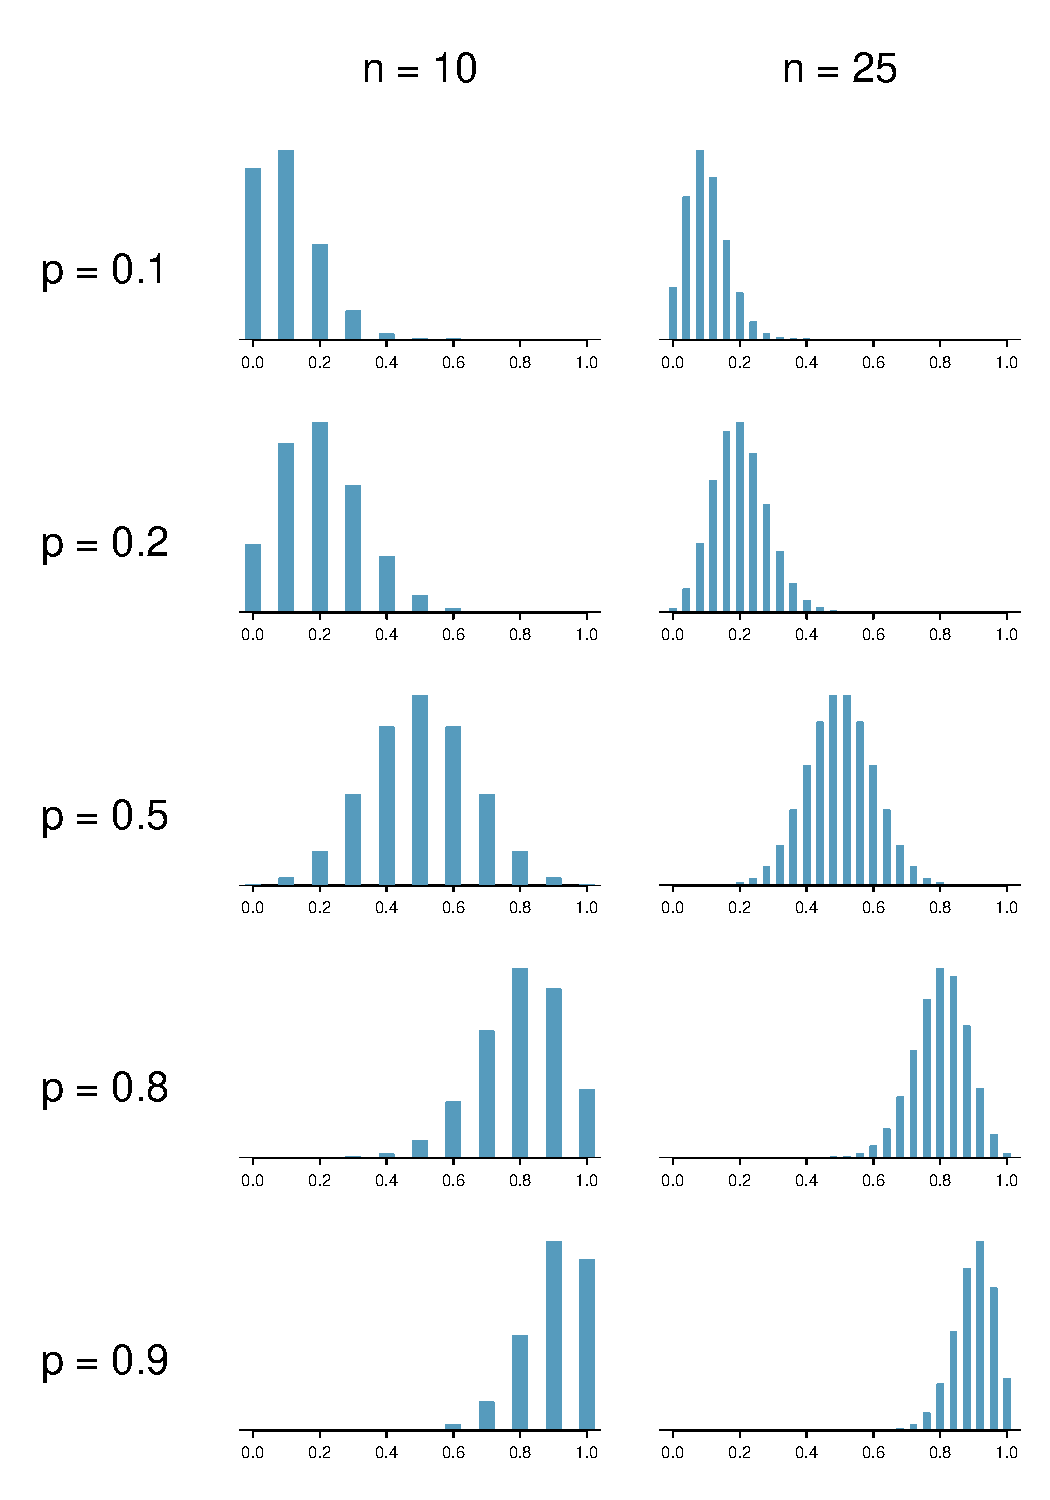
\includegraphics[width=0.45\textwidth]{\chpv@path/5-1_point_est_sampling_var/figures/clt_prop_grid/clt_prop_grid_1.pdf}
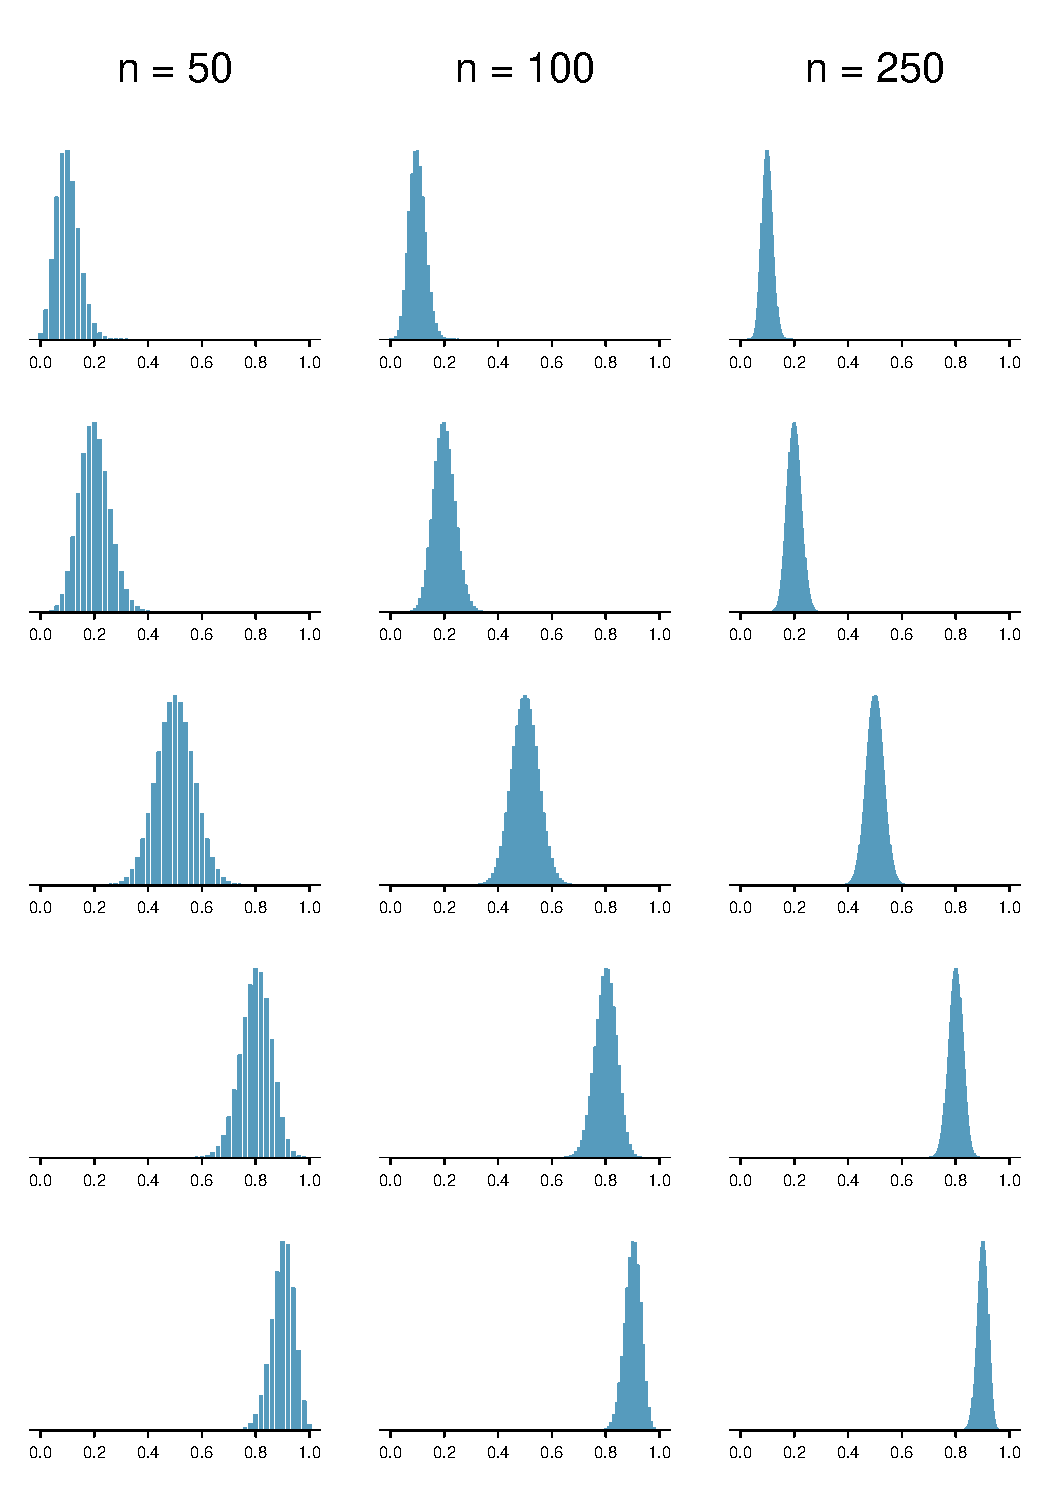
\includegraphics[width=0.45\textwidth]{\chpv@path/5-1_point_est_sampling_var/figures/clt_prop_grid/clt_prop_grid_2.pdf}
\end{center}

\end{frame}

%%%%%%%%%%%%%%%%%%%%%%%%%%%%%%%%%%%

\begin{frame}
\frametitle{When the conditions are not met...}

\begin{itemize}

\item When either $np$ or $n(1-p)$ is small, the distribution is more discrete.
\item When $np$ or $n(1-p)$ $<$ 10, the distribution is more skewed.
\item The larger both $np$ and $n(1-p)$, the more normal the distribution.
\item When $np$ and $n(1-p)$ are both very large, the discreteness of the distribution is hardly evident, and the distribution looks much more like a normal distribution.

\end{itemize}

\end{frame}

%%%%%%%%%%%%%%%%%%%%%%%%%%%%%%%%

\begin{frame}
\frametitle{CLT for the sample mean}

\formula{Central limit theorem (sample mean)}
{Sample means will be nearly normally distributed with mean equal to the population mean, $\mu$, and standard error equal to $\frac{\sigma}{\sqrt{n}}$.
\[ \bar{X} \sim N \pr{ mean = \mu, SE = \frac{\sigma}{\sqrt{n}} } \]
}

\begin{itemize}
    \item This is exactly true if the population distribution is Normal, regardless of sample size $n$ (we derived this in Lecture 16)
    \item But it is also true \emph{regardless of the shape of the population distribution}, as long as the sample size $n$ is sufficiently large.
    \item Different distributions will require different sample sizes for the CLT to ``kick in''.
    \item This is the topic of Lab 5, and we will revisit it in more detail in Chapter 7.
\end{itemize}

\end{frame}
%%%%%%%%%%%%%%%%%%%%%%%%%%%%%%%%%%%%

%%%%%%%%%%%%%%%%%%%%%%%%%%%%%%%%%%%%

\subsection{Extending the framework for other statistics}

%%%%%%%%%%%%%%%%%%%%%%%%%%%%%%%%%%%%

\begin{frame}
\frametitle{Extending the framework for other statistics}

\begin{itemize}

\item The strategy of using a sample statistic to estimate a parameter is quite common, and it's a strategy that we can apply to other statistics besides a proportion or a mean.

\item The principles and general ideas from this chapter apply to other parameters as well, even if the details change a little. 
\begin{itemize}
    \item Using statistics (functions of data) to estimate parameters (population values)
    \item Modeling the sampling process and the statistic using probability tools
    \item Deriving or Simulating the sampling distribution of the statistic
    \item Evaluating bias (is the mean of the sampling distribution equal to the parameter?)
    \item Evaluating variability (how does the standard error change with sample size?)
\end{itemize}
\end{itemize}
\end{frame}

%%%%%%%%%%%%%%%%%%%%%%%%%%%%%%%%%%%%

\section{Confidence intervals for a proportion}

%%%%%%%%%%%%%%%%%%%%%%%%%%%%%%%%%%%%

\subsection{Capturing the population parameter}

%%%%%%%%%%%%%%%%%%%%%%%%%%%%%%%%%%%%

\begin{frame}[shrink]
\frametitle{Confidence intervals}

\begin{itemize}

\item A plausible range of values for the population parameter is called a \hl{confidence interval}.

\item Using only a sample statistic to estimate a parameter is like fishing in a murky lake with a spear, and using a confidence interval is like fishing with a net.
$\:$ \\
$\:$ \\
\begin{columns}[c]
\column{0.25\textwidth}
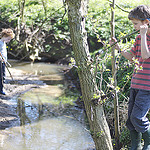
\includegraphics[width=\textwidth]{\chpv@path/5-2_ci_prop/figures/spear}
\column{0.5\textwidth}
{\small
We can throw a spear where we saw a fish but we will probably miss. If we toss a net in that area, we have a good chance of catching the fish.
}
\column{0.25\textwidth}
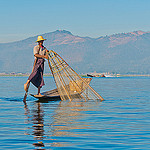
\includegraphics[width=\textwidth]{\chpv@path/5-2_ci_prop/figures/net}
\end{columns}
$\:$ \\
\item If we report a point estimate, we probably won't hit the exact population parameter. If we report a range of plausible values we have a good shot at capturing the parameter. 

\end{itemize}

{\tiny Photos by Mark Fischer (http://www.flickr.com/photos/fischerfotos/7439791462) and Chris Penny (http://www.flickr.com/photos/clearlydived/7029109617) on Flickr.}

% spear fig: http://www.flickr.com/photos/clearlydived/7029109617/sizes/q/
% net fig: http://www.flickr.com/photos/fischerfotos/7439791462/sizes/q/

\end{frame}

%%%%%%%%%%%%%%%%%%%%%%%%%%%%%%%%%%%%

\subsection{Constructing a 95\% confidence interval}

%%%%%%%%%%%%%%%%%%%%%%%%%%%%%%%%%%%%

\begin{frame}
\frametitle{Facebook's categorization of user interests}

\dq{Most commercial websites (e.g. social media platforms, news outlets, online retailers) collect a data about their users' behaviors and use these data to deliver tageted content, recommendations, and ads. To understand whether Americans think their lives line up with how the algorithm-driven classification systems categorizes them, Pew Research asked a representative sample of 850 American Facebook users how accurately they feel the list of categories Facebook has listed for them on the page of their supposed interests actually represents them and their interests. 67\% of the respondents said that the listed categories were accurate. Estimate the true proportion of American Facebook users who think the Facebook categorizes their interests accurately.}

\ct{\webURL{https://www.pewinternet.org/2019/01/16/facebook-algorithms-and-personal-data/}}

\end{frame}

%%%%%%%%%%%%%%%%%%%%%%%%%%%%%%%%%%%%

\begin{frame}
\frametitle{Facebook's categorization of user interests}

\[ \hat{p} = 0.67 \qquad n = 850 \]

\pause

The approximate 95\% confidence interval is defined as 
\[ point~estimate \pm 1.96 \times SE \]

\pause

\vspace{-0.3cm}
\[ SE = \sqrt{\frac{p(1-p)}{n}} = \sqrt{\frac{0.67 \times 0.33}{850}} \approx 0.016 \]

\pause

\vspace{-0.3cm}
\begin{eqnarray*}
\hat{p} \pm 1.96 \times SE &=& 0.67 \pm 1.96 \times 0.016 \\
\pause
&=& (0.67 - 0.03, 0.67 + 0.03) \\
\pause
&=& (0.64, 0.70)
\end{eqnarray*}
\pause

\vspace{-3em}
\Note{Here, we have used the sample proportion $\hat{p}$ in the standard error formula, since we don't have the population proportion $p$.}

\end{frame}

%%%%%%%%%%%%%%%%%%%%%%%%%%%%%%%%%%%

\begin{frame}
\frametitle{}

\pq{Which of the following is the correct interpretation of this confidence interval?}

We are 95\% confident that
\begin{enumerate}[(a)]
\item 64\% to 70\% of American Facebook users in this sample think Facebook categorizes their interests accurately.
\solnMult{64\% to 70\% of all American Facebook users think Facebook categorizes their interests accurately}
\item there is a 64\% to 70\% chance that a randomly chosen American Facebook user's interests are categorized accurately.
\item there is a 64\% to 70\% chance that 95\% of American Facebook users' interests are categorized accurately.
\end{enumerate}

\end{frame}

%%%%%%%%%%%%%%%%%%%%%%%%%%%%%%%%%%%

\begin{frame}
\frametitle{What does 95\% confident mean?}

\begin{itemize}

\item Suppose we took many samples and built a confidence interval from each sample using the equation $point~estimate \pm 1.96 \times SE$.

\item Then about 95\% of those intervals would contain the true population proportion ($p$). 

\end{itemize}

\end{frame}

%%%%%%%%%%%%%%%%%%%%

\section{Edfinity quiz}

%%%%%%%%%%%%%%%%%%%%%%%%%%%%%%%%%%%

\begin{frame}
\frametitle{Width of an interval}

\dq{If we want to be more certain that we capture the population parameter, i.e. increase our confidence level, should we use a wider interval or a smaller interval?}

\pause

\soln{A wider interval.}

$\:$ \\

\pause

\dq{Can you see any drawbacks to using a wider interval?}
\begin{center}

\includegraphics[width=0.9\textwidth]{\chpv@path/5-2_ci_prop/figures/garfield}
\end{center}

\pause

\soln{If the interval is too wide it may not be very informative.}

{\scriptsize Image source: http://web.as.uky.edu/statistics/users/earo227/misc/garfield\_weather.gif}

\end{frame}

%%%%%%%%%%%%%%%%%%%%%%%%%%%%%%%%%%%

% \section{R demonstration: Facebook example}

% %%%%%%%%%%%%%%%%%%%%%%%%%%%%%%%%%%%%

% \subsection{Changing the confidence level}

% %%%%%%%%%%%%%%%%%%%%%%%%%%%%%%%%%%%

% \begin{frame}
% \frametitle{Changing the confidence level}

% \[ point~estimate\pm z^\star \times SE \] 

% \begin{itemize}

% \item In a confidence interval, $z^\star \times SE$ is called the \hl{margin of error}, and for a given sample, the margin of error changes as the confidence level changes.

% \item In order to change the confidence level we need to adjust $z^\star$ in the above formula.

% \item Commonly used confidence levels in practice are 90\%, 95\%, 98\%, and 99\%.

% \item For a 95\% confidence interval, $z^\star = 1.96$.

% \item However, using the standard normal ($z$) distribution, it is possible to find the appropriate $z^\star$ for any confidence level.

% \end{itemize}

% \end{frame}

% %%%%%%%%%%%%%%%%%%%%%%%%%%%%%%%%%%%%

% \begin{frame}

% \pq{Which of the below Z scores is the appropriate $z^\star$ when calculating a 98\% confidence interval?}

% \begin{multicols}{2}
% \begin{enumerate}[(a)]
% \item $Z = 2.05$
% \item $Z = 1.96$
% \solnMult{$Z = 2.33$}
% \item $Z = -2.33$
% \item $Z = -1.65$
% \item[]
% \end{enumerate}
% \end{multicols}

% \soln{\only<2>{
% \begin{center}
% 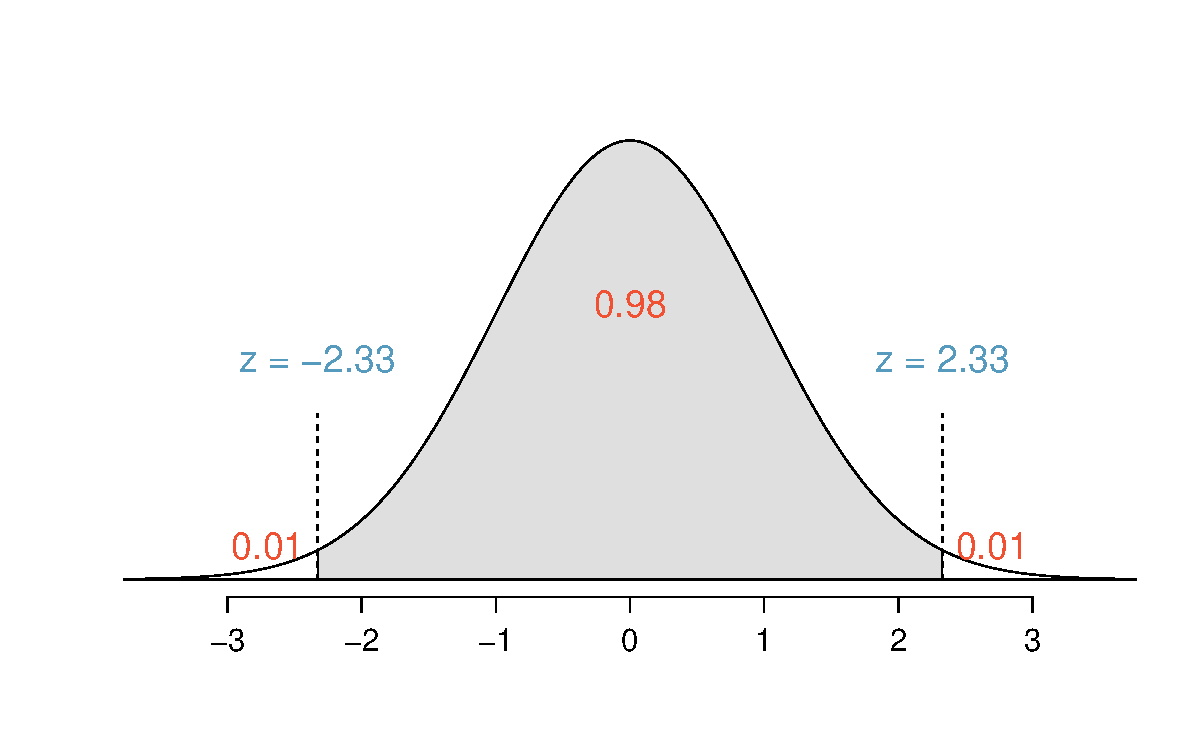
\includegraphics[width=0.7\textwidth]{\chpv@path/5-2_ci_prop/figures/middle98/middle98}
% \end{center}
% }}

% \end{frame}

% %%%%%%%%%%%%%%%%%%%%%%%%%%%%%%%%%%%

% \subsection{Interpreting confidence intervals}

% %%%%%%%%%%%%%%%%%%%%%%%%%%%%%%%%%%%

% \begin{frame}
% \frametitle{Interpreting confidence intervals}

% Confidence intervals are ...

% \begin{itemize}

% \item always about the population

% \item not probability statements 

% \item only about population parameters, not individual observations

% \item only reliable if the sample statistic they're based on is an unbiased estimator of the population parameter

% \end{itemize}

% \end{frame}

% %%%%%%%%%%%%%%%%%%%%%%%%%%%%%%%%%%%

% \section{R demonstration: Effect of confidence level}

%%%%%%%%%%%%%%%%%%%%%%%%%%%%%%%%%%%%

%%%%%%%%%%%%%%%%%%%%%%%%%%%%%%%%%%%%
% End document
%%%%%%%%%%%%%%%%%%%%%%%%%%%%%%%%%%%%

\end{document}